\clearpage
%//==============================--@--==============================//%
\subsection[2.4 Domain Name System (DNS)]{\hspace*{0.075 em}\raisebox{0.2 em}{$\pmb{\drsh}$} Domain Name System (DNS)}
\label{subsec:dns}

The Domain Name System (DNS) is a hierarchical and distributed database that translates human-readable domain names (e.g., \url{www.example.com}) into their corresponding IP addresses, which are used by computers to communicate with each other. This translation is \underline{essential for} the functioning of \underline{the Internet}.

%//==============================--@--==============================//%
\subsubsection[2.4.1 Services Provided by DNS]{$\pmb{\rightarrow}$ Services Provided by DNS}

DNS provides various services, including:

\vspace{-0.5em}
\begin{enumerate}
    \item \textbf{Hostname-to-IP address translation:} The primary function of DNS is to translate domain names into their corresponding IP addresses.
    \item \textbf{Alias resolution:} DNS allows the use of aliases (alternative domain names) to reference the same IP address. This is helpful for load balancing and providing user-friendly names.
    \item \textbf{Reverse lookup:} DNS can perform a reverse lookup, \underline{converting an IP} address back into its \underline{corresponding domain name}.
    \item \textbf{Load distribution:} DNS can distribute the load among multiple servers by returning different IP addresses for the same domain name.
\end{enumerate}

%//==============================--@--==============================//%
\subsubsection[2.4.2 Overview of how DNS works]{$\pmb{\rightarrow}$ Overview of how DNS works}

DNS operates using a distributed hierarchy of servers organized into four levels:

\vspace{-0.5em}
\begin{enumerate}
    \item \textbf{Root DNS servers:} These servers are at the top of the hierarchy and provide information about top-level domains (e.g., .com, .org).
    \item \textbf{Top-level domain (TLD) servers:} These servers are responsible for specific top-level domains, such as .com or .org, and provide information about second-level domains (e.g., example.com).
    \item \textbf{Authoritative DNS servers:} These servers store the actual DNS records for specific domain names and are responsible for providing the IP address associated with a given domain name.
    \item \textbf{Local DNS servers:} These servers are operated by ISPs or organizations and are the first point of contact for end-user DNS queries. They cache query results to provide faster responses for future requests.
\end{enumerate}

\noindent When a user requests the IP address for a domain name, the local DNS server initiates a series of queries through the DNS hierarchy until it reaches the authoritative DNS server for the requested domain, which provides the IP address.

\begin{figure}[H]
    \begin{subfigure}[b]{0.5\linewidth}%
        \centering
        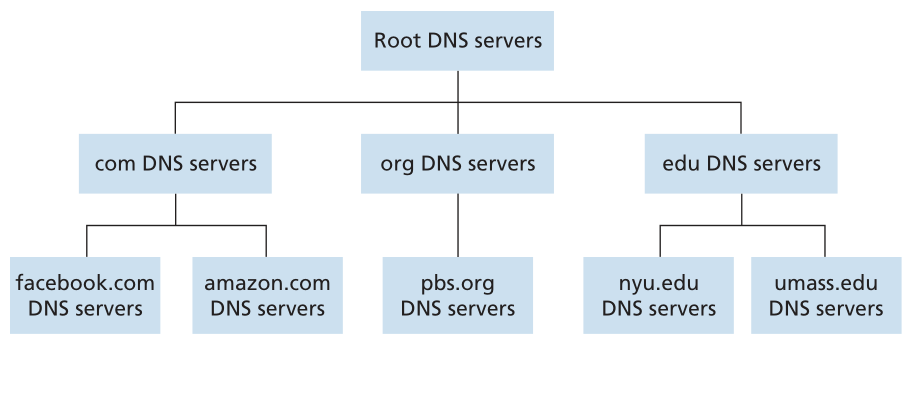
\includegraphics[width = 1\linewidth]{img/2/dns-hierarchy.png}
        \caption{``Portion of the hierarchy of DNS servers''\protect\cite{Kurose2017}}
        \label{fig:dns-hierarchy}
    \end{subfigure} \hfill
    \begin{subfigure}[b]{0.5\linewidth}%
        \centering
        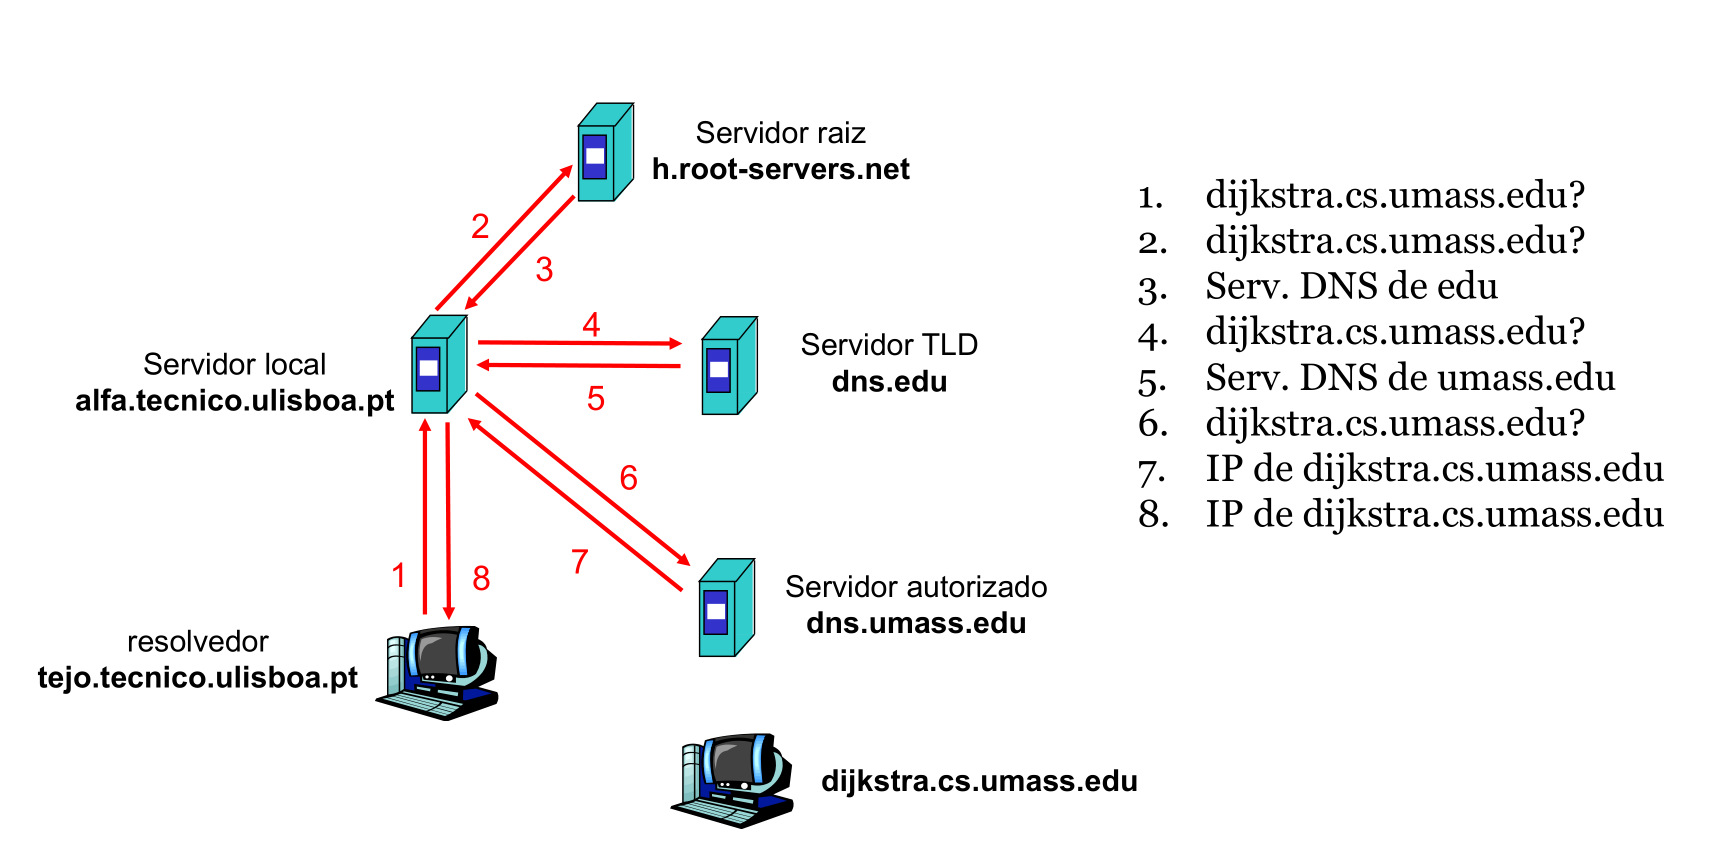
\includegraphics[width = 1\linewidth]{img/2/dns-hierarchy-example.png}
        \caption{``DNS: exemplo''\protect\cite{slidesSobrinho}}
        \label{fig:dns-hierarchy-example}
    \end{subfigure}%
    \caption{DNS hierarchy overview}
\end{figure}

%//==============================--@--==============================//%
\subsubsection[2.4.3 DNS records and messages]{$\pmb{\rightarrow}$ DNS records and messages}

DNS uses \textbf{Resource Records} (RRs) to store information. The most common RR types are:

\vspace{-0.5em}
\begin{enumerate}
    \item \textbf{A:} Contains the IP address corresponding to a given domain name.
    \item \textbf{NS:} Specifies the authoritative name server for a domain.
    \item \textbf{CNAME:} Defines an alias for a domain name, allowing multiple names to reference the same IP address.
    \item \textbf{MX:} Indicates the mail exchange server responsible for handling email for a domain.
    \item \textbf{PTR:} Provides reverse lookup functionality, mapping an IP address back to a domain name.

\end{enumerate}

\begin{lstlisting}[language=, title={Exemplo de registo de recursos \protect\cite{slidesSobrinho}}, frame=tb, basicstyle=\scriptsize\ttfamily, escapechar=\%]
%\begin{center} \small (Domain name, Value, Type, Classe, TTL) \end{center}%

(tejo.tecnico.ulisboa.pt, 193.136.138.142, A, IN, 448)
(tejo.tecnico.ulisboa.pt, 2001:CD00:0:CDE:1257:0:211E:729C, AAAA, IN, 448)
(tecnico.ulisboa.pt, ns1.tecnico.ulisboa.pt, NS, IN, 3600)
(mae.princeton.edu, live-princeton-mae-next.pantheonsite.io, CNAME, IN, 86400)
(tecnico.ulisboa.pt, email.tecnico.ulisboa.pt, MX, IN, 3600)
\end{lstlisting}

\vskip 0.5em
\noindent DNS messages consist of two types of messages:

\vspace{-0.5em}
\begin{enumerate}
    \item \textbf{Query:} A message sent by a client (local DNS server) to a DNS server, requesting the resolution of a domain name or an IP address.
    \item \textbf{Response:} A message sent by the DNS server back to the client, containing the requested information (e.g., IP address or domain name) and any additional relevant records.
\end{enumerate}

\noindent Both query and response messages have the same format, consisting of a header and four sections: Question, Answer, Authority, and Additional Information. The header contains various flags and identifiers, while the four sections contain the relevant resource records and requested information.

\begin{figure}[H]
    \centering
    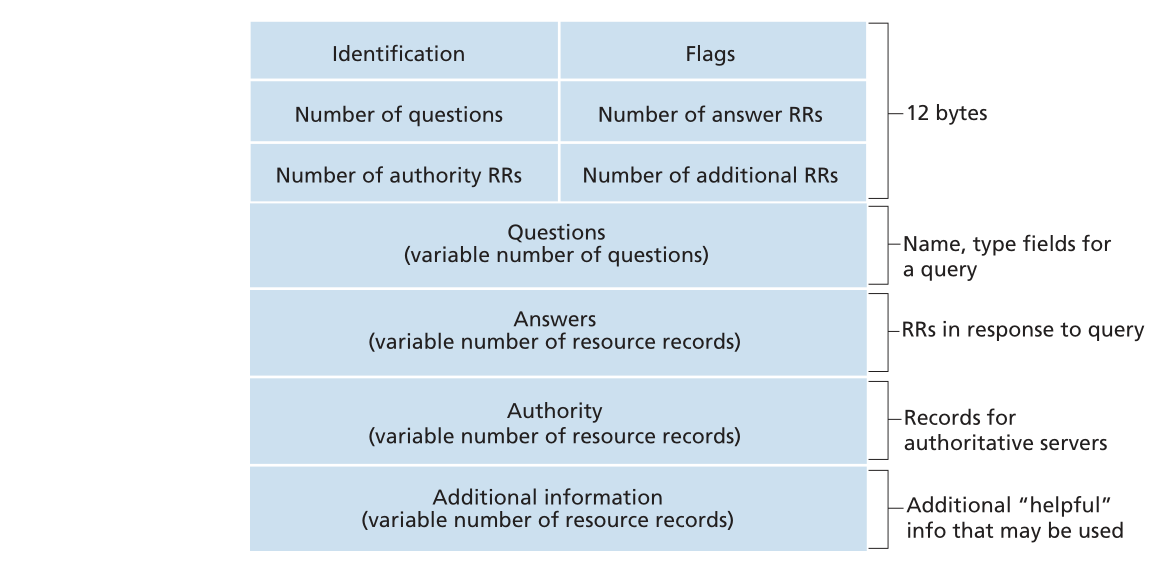
\includegraphics[width = 0.8\linewidth]{img/2/dns-message-format.png}
    \caption{``DNS message format''\protect\cite{Kurose2017}}
    \label{fig:dns-message-format}
\end{figure}

\renewcommand*{\thefootnote}{\fnsymbol{footnote}}
\footnotetext[4]{%
``\texttt{TTL} is the Time-To-Live of the resource record; it determines when a resource should be removed from a cache.''\cite{Kurose2017}
}
\renewcommand*{\thefootnote}{\arabic{footnote}}

%//==============================--@--==============================//%
\subsubsection[2.4.4 DNS Caching and Query Resolution]{$\pmb{\rightarrow}$ DNS Caching and Query Resolution}


\begin{enumerate}
    \item \textbf{DNS Caching:} Temporarily storing DNS query results to reduce lookup times for subsequent requests.
    \begin{enumerate}
            \item \textbf{Local Cache:} DNS clients (resolvers) and recursive DNS servers store query results locally to quickly answer repeated requests.
            \item \textbf{Cache Expiration:} Each DNS record has a Time-To-Live (TTL) value determining how long it should be stored in a cache before being discarded.
    \end{enumerate}
    
    \item \textbf{Recursive Query:} A DNS server contacts other DNS servers on behalf of the client to resolve a query, returning the final result to the client.
    
    \item \textbf{Iterative Query:} A DNS server provides the client with a referral to another DNS server, and the client continues the query resolution process by contacting the referred server.
\end{enumerate}

%//==============================--@--==============================//%